\section{Ecosystem Architecture}

\subsection{Ecosystem Overview}
The Craftalism ecosystem is composed of multiple independent modules that work together to provide a persistent and observable economic system for Minecraft servers. Each module has a clearly defined responsibility and communicates with others through well-defined interfaces. This modular structure allows gameplay logic, data persistence, visualization, and infrastructure concerns to evolve independently while remaining loosely coupled.

This section describes how these modules are structured, how they interact, and how data flows across the ecosystem.

\begin{figure}[H]
	\centering
	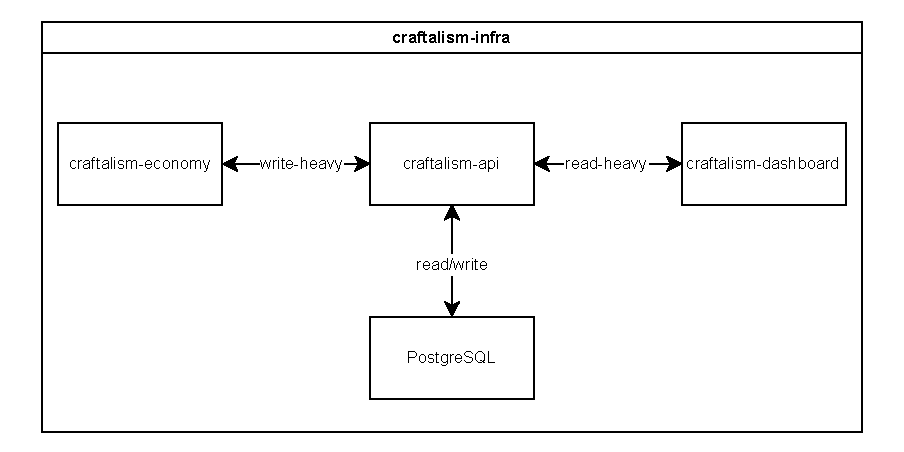
\includegraphics[width=0.8\textwidth]{assets/ecosystem-architecture-diagram.pdf}
	\caption{Craftalism ecosystem architecture}
	\label{fig:architecture}
\end{figure}